\section{Demografis indflydelse på vurderinger}
\label{sec:Demografi}
%
I dette afsnit beskrives hvordan forskellene mellem testpersonerne kan være med til at påvirke vurderingen af robotten. Der fokuseres isoleret på hvordan de demografiske faktorer påvirker hver enkelte skala. Det er valgt kun at medtage de grafer, hvor der forekommer en tendens for korrelation mellem alder og besvarelser til skalaerne. Dog er analysen foretaget på tværs af alle demografiske faktorer og samtlige skalaer, med undtagelse af hvor ofte testpersonerne rejser. Årsagen til at analysen ikke foretages i forhold til hvor ofte testpersonerne rejser skyldes hovedsageligt én ting, at AAL er relativt lille lufthavn, hvor der formentlig ikke er et lige så stort behov for robottens hjælp, som eksempelvis kan være tilfældet i Københavns Lufthavn. Med det i betragtning antages det, at for rejsende, som rejser privat flere gange årligt eller som rejser i forbindelse med arbejde, formentlig ikke adskiller sig specielt meget. Hvorimod hvis undersøgelsen blev foretaget i en større lufthavn, så kan det sagtens være at der er en forskel. Dette kan formentlig have særlig betydning for testpersonernes vurdering i forhold til hvorvidt de føler, at robotten kan hjælpe dem, om de stoler på, at den følger dem det rigtige sted hen, om den står i vejen og hvorvidt robotten opleves som værende anmassende.\blankline
% 
I henhold til testpersonernes alder tyder det på, at der er en positiv korrelation mellem alder og SQ6, jævnfør \autoref{fig:AgeSQ6}. Der er derfor en tendens til at desto ældre testpersonerne er, desto mere synes de, at robotten kører for hurtigt. 
%
\begin{figure}[H]
\centering
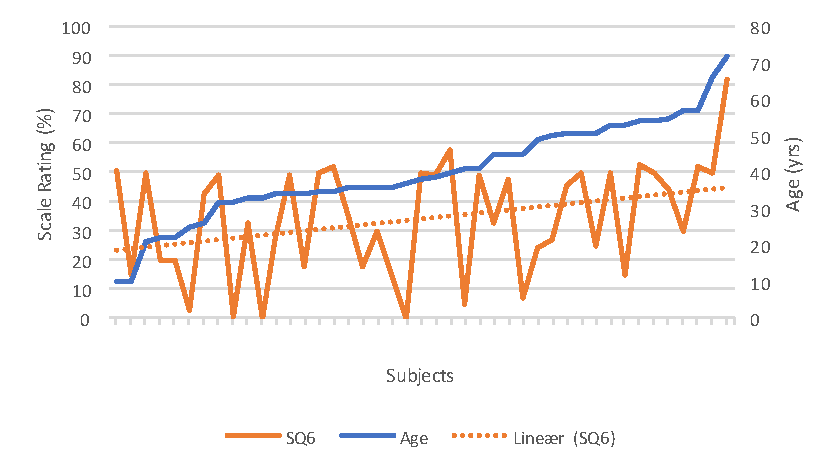
\includegraphics[width=\textwidth]{Figure/DatabehandlingSkalaer/Demografi/AgeSQ6}
\caption{Sammenhæng mellem hvad testpersonerne angiver (\%) på skalaen til SQ6: \textit{Jeg synes, at robottens hastighed er...}, og deres alder. Denne graf bygger på samtlige besvarelser.}
\label{fig:AgeSQ6}
\end{figure}
\noindent
%
Derudover forekommer der en lille negativ korrelation mellem testpersonernes alder og hvor spændende de synes robotten er, jævnfør \autoref{fig:AgeSQ18}. Der er derfor en tendens til at desto ældre testpersonerne, desto mindre spændende synes de, at robotten er. Derudover tyder det på at testpersoner mellem 35 år og 45 år finder robotten mindst spændende.
%
\begin{figure}[H]
\centering
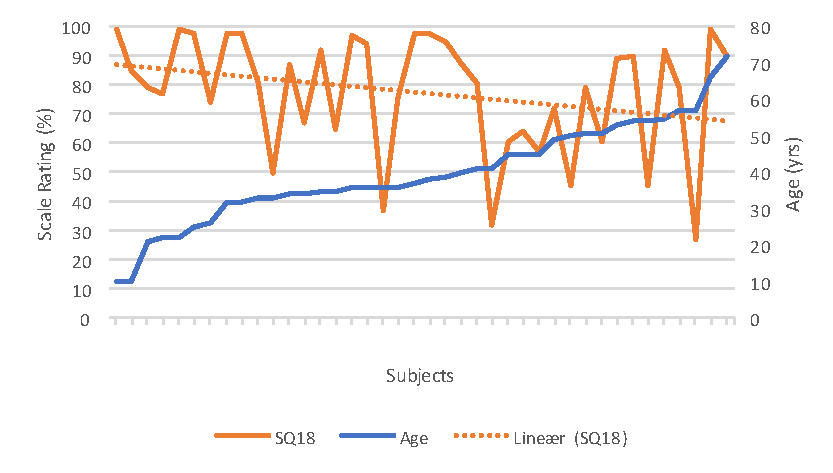
\includegraphics[width=\textwidth]{Figure/DatabehandlingSkalaer/Demografi/AgeSQ18}
\caption{Sammenhæng mellem hvad testpersonerne angiver (\%) på skalaen til SQ18: \textit{Hvad synes du om robotten?}, i forhold til \textit{spændende}, og deres alder. Denne graf bygger på 40 besvarelser, da der manglede tre.}
\label{fig:AgeSQ18}
\end{figure}
\noindent
%
Lignende forefindes mellem testpersonernes alder og SQ22, vedrørende hvor sjov robotten opleves, hvor der en lille tendens til en negativ korrelation, hvilket fremgår af \autoref{fig:AgeSQ22}. Det tyder på at desto ældre testpersonerne er, desto mindre sjov synes de, at robotten er. 
%
\begin{figure}[H]
\centering
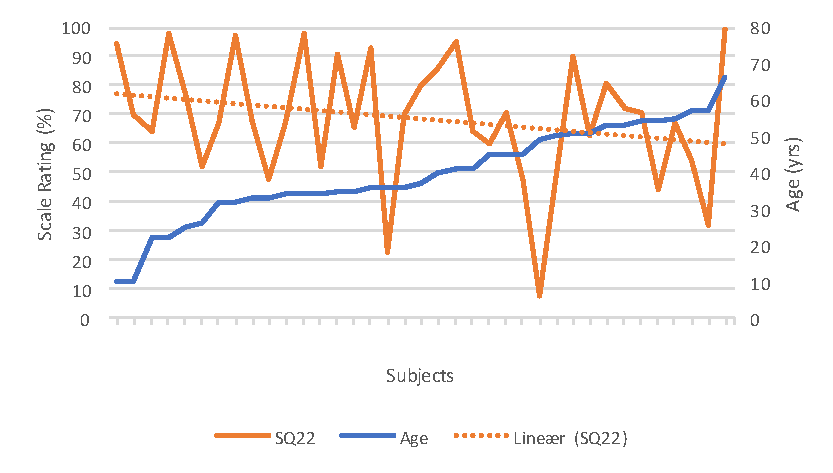
\includegraphics[width=\textwidth]{Figure/DatabehandlingSkalaer/Demografi/AgeSQ22}
\caption{Sammenhæng mellem hvad testpersonerne angiver (\%) på skalaen til SQ22: \textit{Hvad synes du om robotten?}, i forhold til \textit{sjov}, og deres alder. Denne graf bygger på 37 besvarelser, da der manglede seks.}
\label{fig:AgeSQ22}
\end{figure}
\noindent
%



\fxnote{Passer muligvis bedre ind under robothøjde} Vi kan se at jo større højdeforskellen er mellem menneske og robot, jo sødere og mere elegant opleves robotten. \autoref{fig:heightRatio19}. Det betyder altså at en robotten opleves sødere og mere elegant, jo lavere den er i forhold til brugeren, da de fleste testpersoner var højere end robotten.

\begin{figure}[H]
\centering
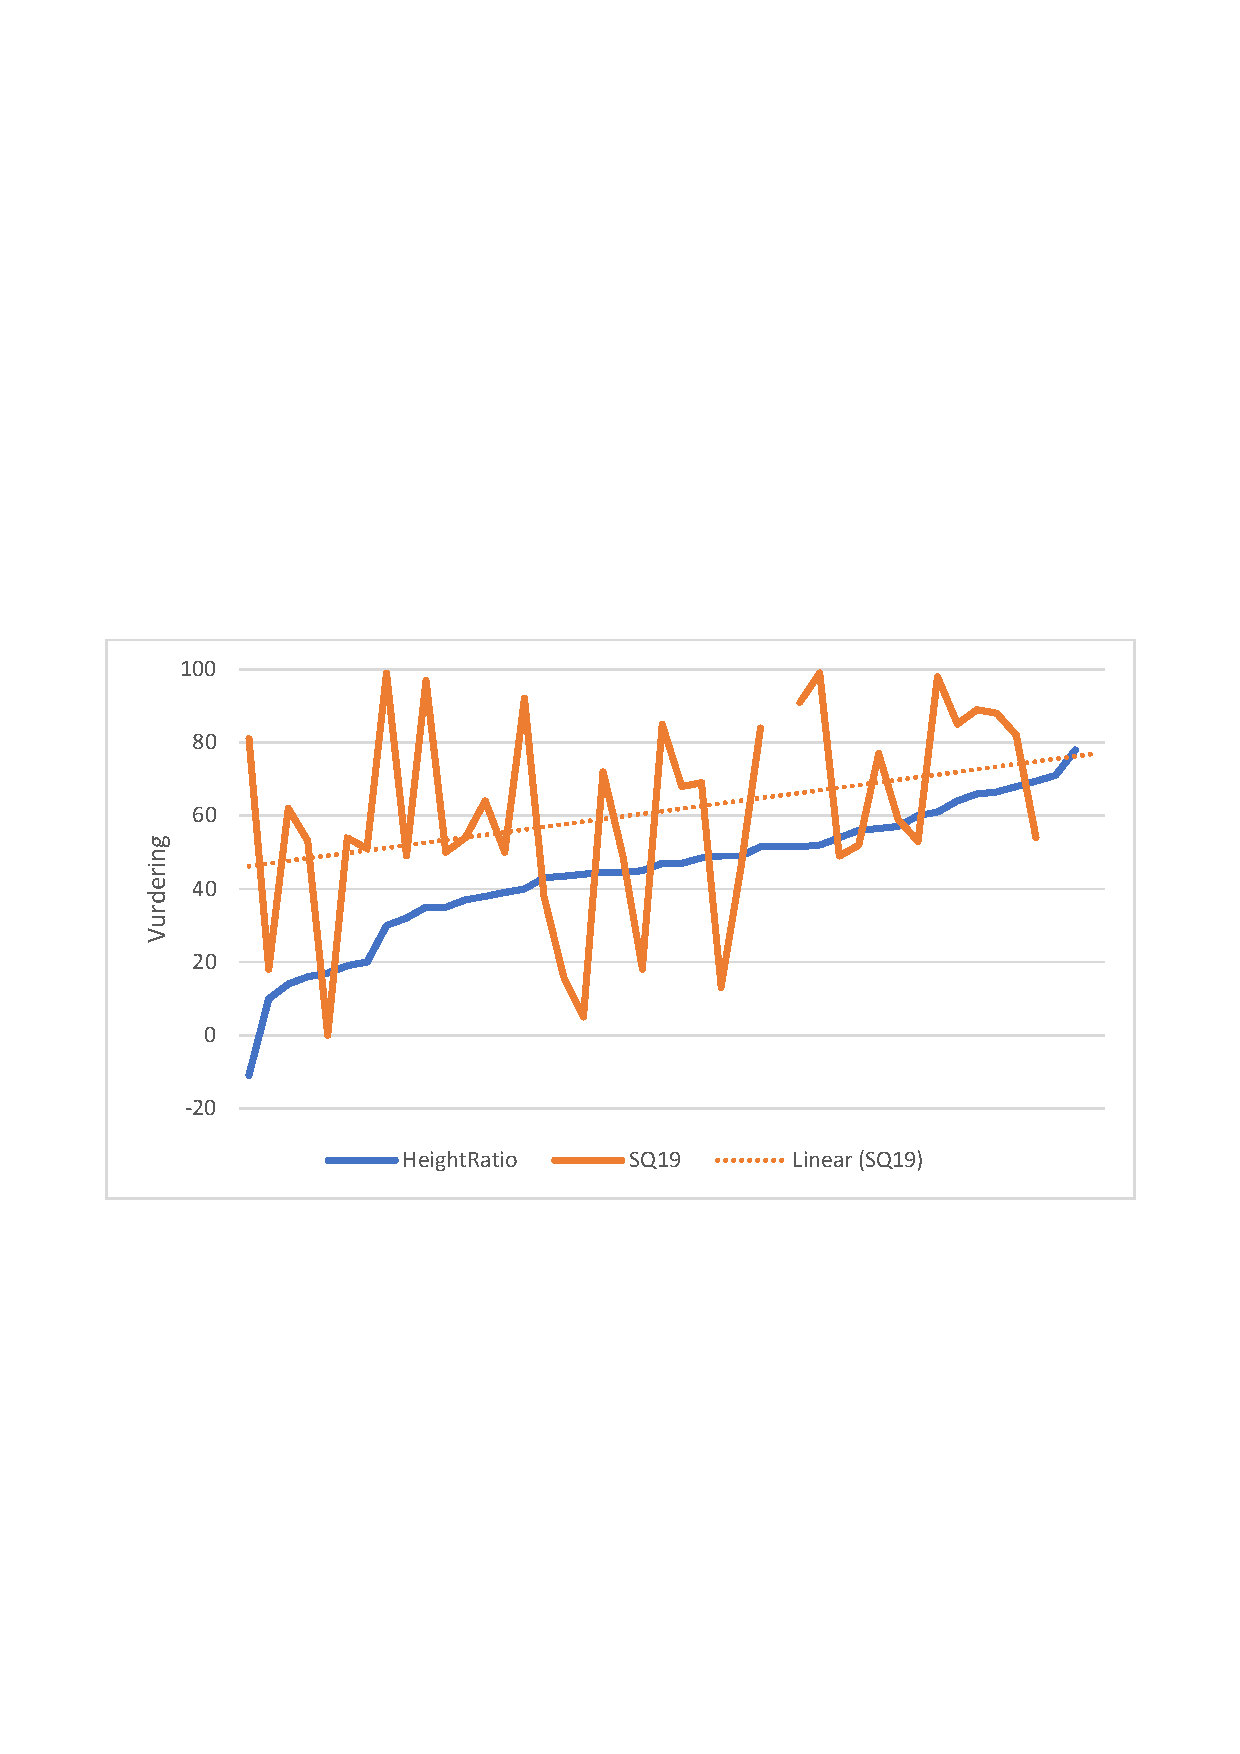
\includegraphics[width=\textwidth]{Figure/DatabehandlingSkalaer/Demografi/HeightRatio.pdf}
\caption{}
\label{fig:heightRatio19}
\end{figure}
\noindent

Robotten opleves også hurtigere og vildere, når den er lav, hvilket giver god mening, da robotten rent faktisk kører hurtigere ved de lave højder \autoref{fig:heightRatio4_6}.


\begin{figure}[H]
\centering
\includegraphics[width=\textwidth]{Figure/DatabehandlingSkalaer/Demografi/HeightRatio4_6.png}
\caption{}
\label{fig:heightRatio4_6}
\end{figure}
\noindent


Der var meget stor forskel på hvor godt skærmen reagerede, og der var ikke nogle af faktorerne som beskrev hvad denne forskel kom af. For eksempel var dem som var glade for teknologi ikke bedre til at trykke rigtigt på skærmen.

Vi kan se at der er svaret lige omkring midten for spørgsmål 5 og 7 på tværs af alle de demografiske faktorer. 5 og 7 er derfor ikke særligt beskrivende for den oplevelse folk har haft, da alle har svaret cirka det samme både på tværs af demografi og på tværs af de stimuli de har været udsat for (forskellige højder, afstande og vinkler). 5=robotten er for tæt på/langt væk, 7=robotten er for høj/lav.